\documentclass[11pt,a4paper]{ltjsarticle}
% Compile with LuaLaTeX

% =========================
% Packages
% =========================
\usepackage{luatexja}
\usepackage{graphicx}
\usepackage{hyperref}
\usepackage{amsmath,amssymb,mathtools}
\usepackage{xcolor}
\usepackage{float}
\usepackage{subcaption}
\usepackage{booktabs}
\usepackage{enumitem}
\usepackage{geometry}

\geometry{margin=22mm}
\setcounter{tocdepth}{3}
\setlength{\parskip}{0.6mm}

% =========================
% User information
% =========================
\title{Weekly Report: Ultra-High-Pressure ODMR --- \\ Is the 475\,nm optimal blue wavelength robust to detection-window background?}
\author{Risei Abe}
\date{Week: 2026/07/26 -- 2026/08/01}

% =========================
% Custom commands
% =========================
\newcommand{\sectionblock}[1]{%
  \vspace{2mm}
  {\large\textbf{#1}}
  \vspace{1mm}

}

\newcommand{\todo}[1]{\textcolor{red}{#1}}

\begin{document}

\maketitle

% =========================================================
% 1. Question / Purpose
% =========================================================
\sectionblock{Question}

\begin{quote}
Our NV-only model puts the optimal blue excitation wavelength at 120\,GPa at $\lambda_{opt}\approx 475$\,nm; does adding a spin-independent background inside the $>650$\,nm detection window shift $\lambda_{opt}$ far enough to change which commercial laser line (473 or 488\,nm) we should order?
\end{quote}

% =========================================================
% 2. Hypothesis
% =========================================================
\sectionblock{Hypothesis}

If the Cr$^{3+}$ transmission gap ($\sim$476\,nm) sits close to the NV-only optimum while N3 background rises toward the near-UV, background should push $\lambda_{opt}$ only slightly to the red, staying inside the existing 5\% sensitivity tolerance band so that the choice between 473\,nm and 488\,nm laser lines is unaffected.

% =========================================================
% 3. Evidence / Interpretation
% =========================================================
\sectionblock{Evidence / Interpretation}

\begin{figure}[H]
  \centering
  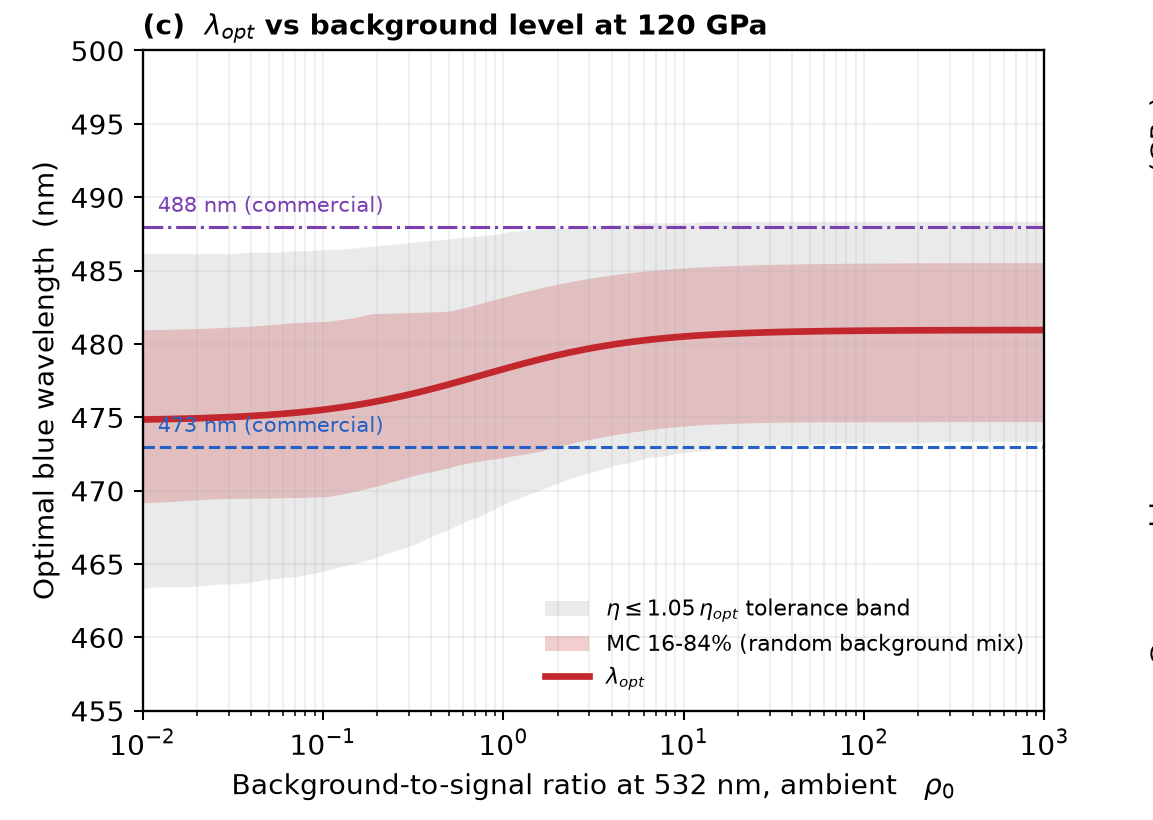
\includegraphics[width=0.46\linewidth]{image/lambda_opt_vs_rho0.png}
  \vspace{-1mm}
  \caption{Optimal blue wavelength $\lambda_{opt}$ vs.\ background level $\rho_0$ at 120\,GPa, with the $\eta\le1.05\,\eta_{opt}$ tolerance band (grey) and a Monte-Carlo 16--84\% band over random background compositions (red shading).}
  \label{fig:lambda_opt}
\end{figure}
\vspace{-3mm}

\begin{itemize}[leftmargin=8mm]
  \item $\lambda_{opt}$ shifts only from 474.8\,nm ($\rho_0{=}0$) to 480.9\,nm ($\rho_0\to\infty$), i.e.\ $<6$\,nm total, and stays inside the zero-background tolerance band [463, 486]\,nm.
  \item The Monte-Carlo band over randomized ruby/N3/broad-luminescence mixing weights spans roughly [465, 487]\,nm across all $\rho_0$, so the conclusion does not depend on which background composition we assume.
\end{itemize}

% =========================================================
% 4.  Gap / Failure
% =========================================================
\sectionblock{Gap / Failure}

\begin{itemize}[leftmargin=8mm]
  \item Both 473\,nm and 488\,nm remain within the tolerance band for every $\rho_0$ tested, so this calculation alone cannot rank the two commercial lines against each other.
  \item The model treats background as wavelength-shape only and ignores any pressure dependence of the ruby/N3 emission strength itself, which could move the gap location at 120\,GPa.
\end{itemize}

% =========================================================
% 5. Next Step
% =========================================================
\sectionblock{Next Step}

Once the background spectrum is measured (see companion report on the crossover question), refit the Cr$^{3+}$/N3 shape parameters to the real anvil and re-run \texttt{fig5\_background.py} to check whether the calibrated $\lambda_{opt}$ still favors 473\,nm over 488\,nm.

% =========================================================
% 9. References
% =========================================================
\sectionblock{References}

\begin{enumerate}[leftmargin=8mm]
  \item K.\,O.\ Ho, C.\ Dailledouze, V.\ \v{Z}alandauskas, \emph{et al.}, ``Optical Stability and Photophysics of NV Centers in Diamond up to 120 GPa,'' arXiv:2606.02399 (2026).
  \item A.\ Dr\'eau \emph{et al.}, Phys.\ Rev.\ B \textbf{84}, 195204 (2011).
  \item Repository: \texttt{code/nv\_bg.py}, \texttt{code/background.py}, \texttt{code/fig5\_background.py} (this analysis).
\end{enumerate}

\end{document}
